\chapter{webs}
\label{sec:webs}
\lstset{style=68KStyle}

Webs are fun and should be easy to draw. To start with, we can describe a 2d shape
of our choice using a bunch of x/y co-ordinates as points.
\begin{figure}[H]
    \centering
    \begin{adjustbox}{width=7cm,center}
      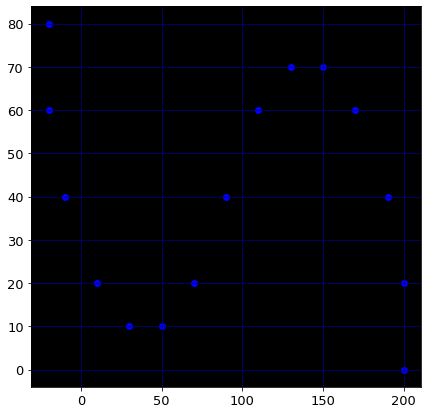
\includegraphics[width=12cm]{src/webs/sine_wave_dots_no_title.png}%
    \end{adjustbox}
  \caption{Make our dots.}
\end{figure}

Next we can join these together to give us a 2d shape.
\begin{figure}[H]
    \centering
    \begin{adjustbox}{width=8cm,center}
      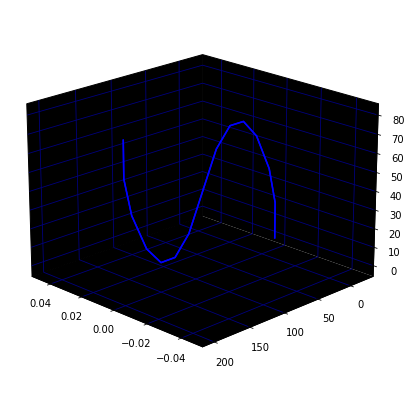
\includegraphics[width=12cm]{src/webs/sine_wave_2d_no_title.png}%
    \end{adjustbox}
  \caption{Start with a 2d shape..}
\end{figure}

To make this thing three dimensional all we have to do is project our shape onto
some chosen distant position along the Z plane.
\vspace{-0.5cm}
\begin{figure}[H]
    \centering
    \begin{adjustbox}{width=8cm,center}
      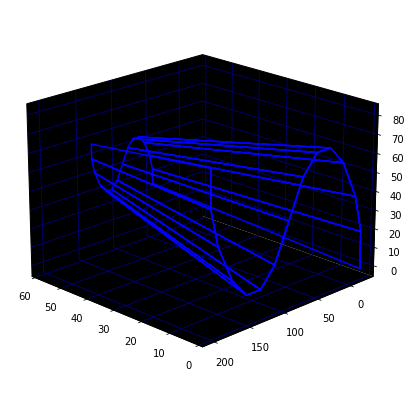
\includegraphics[width=12cm]{src/webs/sine_wave_no_title.png}%
    \end{adjustbox}
  \caption{..then make it three dimensional.}
\end{figure}

Seems simple enough. With this as our objective the data structure below gives us
everything we need to create the web. In addition to listing the 16 vertices that
make up the web's shape in two dimensions, we also include some information on whether
the web should be open (like the one pictured above) or closed (like a circle or 
square). Since a web of 16 vertices will give us 14 lanes which the player and
enemies can occupy we also add a 'Rotation Table' to tell us how players and
enemies should be oriented when on that lane.

\begin{lstlisting}
; Data structure for the 'Sine Wave' web. 
web13:       
  dc.w 14    ; Number of lanes in the web.
  dc.w  6    ; The lane the player starts on.

  ; The x/y pairs of all vertices in the web. So for example
  ; -2/14 indicates the X and Y co-ordinates of the first vertex.
  ; There are always 16 in total.
  dc.w -2,14,-2,12,-1,10, 1, 8
  dc.w  3, 7, 5, 7, 7, 8, 9,10
  dc.w 11,12,13,13,15,13,17,12
  dc.w 19,10,20, 8,20, 6,-2,14

  dc.w 0     ; 0 = Open Web, -1 = Closed Web
    
  ; Rotation Table (angle of an object within a particular lane)
  ; The length of this list is specified by the '14' above.
  dc.w -64,-48,-32,-16, 0,16,32,32,16, 0,-16,-32,-48,-64
\end{lstlisting}

The values given in the Rotation Table are angles of roll to apply to the claw
(and to the claw's enemies) when placing them in the lane. Negative values rotate
the object to the right, while positive values rotate it to the left. 
\begin{figure}[H]
    \centering
    \begin{adjustbox}{width=6cm,center}
      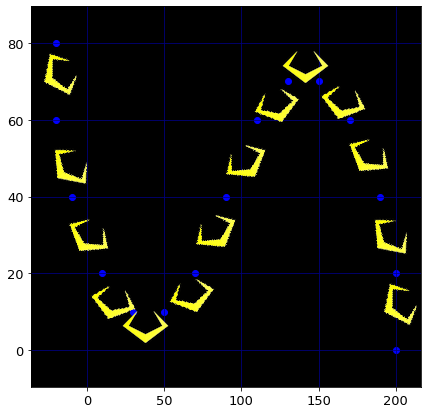
\includegraphics[width=12cm]{src/webs/sine_wave_dots_claws_no_title.png}%
    \end{adjustbox}
  \caption{The rotation table applied to the claw in each lane of the web.}
\end{figure}

This is the routine that converts the web data structure into a list of vertices and lines between vertices
that will make up the web itself:

\begin{lstlisting}
extrude:
;
; extrude a web from a list of 16 pairs of XY coordinates addressed by (a1)
;
; a0 = vector ram space; a2.l = z depth to extrude to; d0-d7 as above

  move.l vadd,a0
  movem.l d0-d7/a0/a2,-(a7)    ;save so routine can return address
  clr connect
  move.l a2,-(a7)    ;save z depth
  bsr initvo    ;make header, do standard vector object init
  move.l a3,a4    ;save first vertex
  move.l (a7)+,d7    ;retrieve z-depth
  move d7,d0
  asr #1,d0
  move d0,web_z    ;Current Web z centering
  clr.l d0
  clr.l d1
  clr d5      ;to catch highest X point
  move (a1)+,d6            ; No of lines in the web.
  move d6,web_max          ; Keep it in web_max
  move (a1)+,web_firstseg  ; first position on web
  move.l a1,web_ptab       ;position table
  move.l a3,(a5)+          ;first vertex to lanes list
\end{lstlisting}

\begin{lstlisting}
  ; Read in the x/y pairs
xweb:
  ; Get the current x and y pair
  move (a1)+,d0
  move (a1)+,d1    ;get X and Y
  ext.l d0
  ext.l d1

  ; Check if this is the large X value so far
  cmp d5,d1       ; Compare x with the largest so far, stored in d5. 
  blt xweb2       ; If it's less, skip to xweb2 below.
  move d1,d5      ; It's bigger, so save it in d5.

xweb2:
  ; Store the x,y,z value for the near point in the web
  move.l d0,(a2)+ ; x value
  move.l d1,(a2)+ ; y value
  clr.l (a2)+     ; z value for near point (always 0)

  ; Store the x,y,z value for the far point in the web
  move.l d0,(a2)+ ; x value
  move.l d1,(a2)+ ; y value
  move.l d7,(a2)+ ; z value for far point (calculated by initvo).

  move d3,(a3)+    ;vertex ID to conn list
  tst d6
  beq lastpoint    ;special case for last point!

  ; Connect the vertices
  move d3,d4       ;copy vertex #
  addq #1,d4
  move d4,(a3)+    ;connect to n+1
  addq #1,d4
  move d4,(a3)+    ;connect to n+2
  move #0,(a3)+    ;end vertex 
  subq #1,d4       ;point to n+1
  move d4,(a3)+
  addq #2,d4       ;n+3
  move d4,(a3)+    ;connect
  move #0,(a3)+    ;delimit
  move.l a3,(a5)+  ;to v.conn list
  add #2,d3        ;move 2 vertices

  ; Get the next pair
  dbra d6,xweb
\end{lstlisting}

\begin{figure}[H]
    \centering
    \begin{adjustbox}{width=9cm,center}
      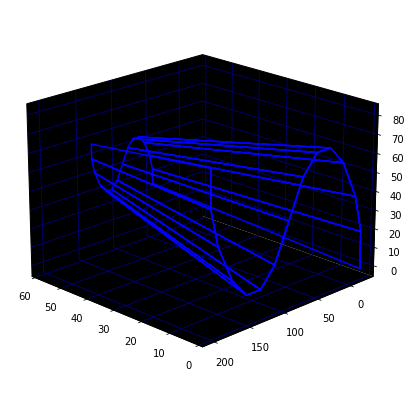
\includegraphics[width=12cm]{src/webs/sine_wave_no_title.png}%
    \end{adjustbox}
  \caption{Adding in our second triangle}
\end{figure}
